\documentclass[12pt,a4paper]{article}%
\usepackage[utf8]{inputenc}

%%%% pour ne pas compiler les images
\usepackage{graphicx}
%\usepackage[draft]{graphicx}

\usepackage{geometry}
\usepackage{a4wide}
\usepackage{ulem}
\usepackage{amsmath}
\usepackage{amsfonts}
\usepackage{amssymb}
\usepackage[T1]{fontenc}%
\setcounter{MaxMatrixCols}{30}
\usepackage{hyperref}
\usepackage{appendix}
 
 
\providecommand{\U}[1]{\protect\rule{.1in}{.1in}}
%EndMSIPreambleData
\usepackage{color}
\renewcommand{\@}{\textcolor{red}}
\newcommand{\ed}{\textsc{EcoDyco}}

\date{}

\begin{document}

\newgeometry{top=20mm,bottom=20mm}
\begin{titlepage}

	\centering
		{\Huge \textbf{--- \ed\ ---} \\[0pt]}
		{\Large Economic Modelling in a World of Finite Resources \\[1cm]}
		\Large Author \textbf{DyCo} \\ 
		\large Universit\'e Paris Cit\'e, CNRS, UMR 8236 \\
		 LIED, F-75013 Paris, France
		\vspace{1cm}

		\begin{figure}[h]
			\centering 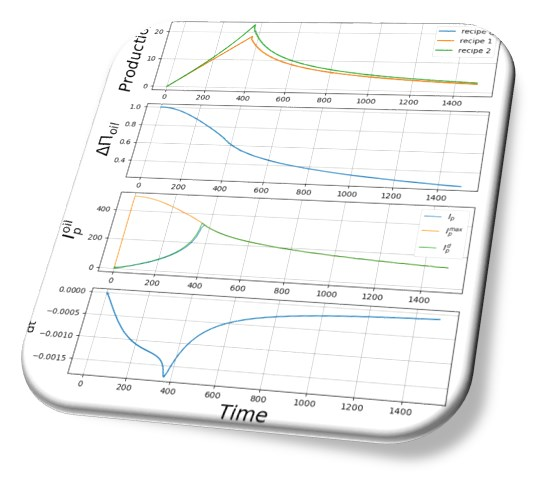
\includegraphics[width=0.9\textwidth]{figures/couverture.jpg}
		\end{figure}
	
		\vspace{1cm}
		{\Huge \textbf{User Manual v0.9} \\[0.5cm]}
		{\Large Sept. 2022 \\[0.5cm]}
		{\large All the material necessary to run the following examples,\\ including this manual, can be found at \url{https://github.com/dyco-uparis/EcoDyco}. 
		}

\end{titlepage}
\restoregeometry

\tableofcontents
\setcounter{page}{1}

\newpage


\section{\ed, Economic Modelling in a World of Finite Resources}

The model \ed\ was designed on the basis of five findings:

\begin{enumerate}
	\item If the physical world is modified by the application of the laws of the economy
	of the economy, the fact remains that its evolution is governed by
	physical laws.
	
	\item The physical world is finite, this is true for all material resources
	resources and for fossil energy resources.
	
	\item In a finite world, the definition of a production function must take into account the state of the resources. Production is contingent on the available resource.
	
	\item The intensity of withdrawal from a resource is a major factor
	on the fate of the resource.
	
	\item If the economy is not strictly describable by thermodynamics,
	thermodynamics can provide it with some useful categories, and in particular the
	In particular, the distinction between \textit{quantity} and \textit{quality},
	themselves linked to the intensive or extensive character of the variables.
\end{enumerate}


\noindent These findings form the basis for the structure and operation of the model \ed.

\begin{enumerate}
	\item The descriptions of the physical and economic spheres of the model
	are disjointed. They communicate through specific variables and parameters. 
	
	\item Each resource is described in its own sheet. The collection of sheets thus obtained is the physical sphere. Each sheet quantifies the usable fraction and the used fraction of the
	Each sheet quantifies the usable fraction and the used fraction of the resource, which we will call waste. The used fraction can only be used again
	used again only after recycling.
	
	\item It is defined a production query function called ``demand'', which
	replaces, for the physical dimension, the production function. The structure and the parameterisation 
	The structure and parameterisation of the production function are fixed by the specific choices
	The structure and parameterisation of the production function are fixed by specific choices made in the economic area of the model.
	
	\item It is defined an intensity of operation of the economy which governs
	the whole of the physical sheets.
	
	\item The quantities of resources are also associated with qualities, which, like the first and second principles, are
	the image of the first and second principles of thermodynamics, define,
	the difference in quality of a resource and its state of transformation, towards a
	transformation, towards a product or towards a waste.
\end{enumerate}


\section{General structure of \ed}

The model is structured in sheets of stock type and flow type,
linked to the economic module. Its overall architecture is shown figure~\ref{fig:globalstructure}.


\begin{figure}[h]
	\centering 
	\includegraphics[width=0.75\textwidth]{figures/Archiglobale.jpg}
	\caption{text}
	\label{fig:globalstructure}
\end{figure}


\subsection{Structure of a Stock sheet}

Stock sheets are intended for most resources, mineral, fossil or not, whose quantity on the planet is finite and of variable dispersion.

\begin{figure}[h]
	\centering
	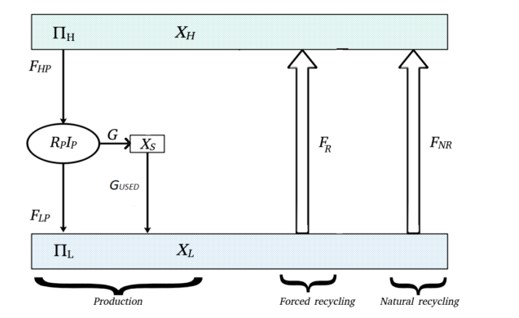
\includegraphics[width=0.75\textwidth]{figures/FeuilleStock.jpg}
	\caption{text}
	\label{fig:StockSheet}
\end{figure}

On a typical stock sheet (figure~\ref{fig:StockSheet}), there is a high zone containing the resource in quantity $X_{H}$ and quality $\Pi_{H}$ and a zone of used resource in quantity $X_{L}$ and quality $\Pi_{L}$. The resource flows of $F_{HP}$ and the waste flows $F_{LP}$ constitute, together with the production flow $G$, the whole of the resource flows in its implementation for production.
The quantity of resource used in excess constitutes a stock $X_{S}$. Recycling can be natural $F_{NR}$, or forced, $F_{R},$ according to specific laws. We call the difference of potentials the quantity $\Delta \Pi=\Pi_{H}-\Pi_{L}$.



\subsubsection{Stock sheet parameters}

A stock sheet is initially defined by the set of limited parameters listed below, values are given as an example.

\begin{itemize}
\item \textit{type : stock}

\item \textit{name : copper}

\item Total quantity --- \textit{total stock : 500000}

\item Initial quantity of high level --- \textit{Xh\_init : 500000}

\item Initial quantity of sink --- \textit{Xl\_init : 0}

\item Production dissipation resistance --- \textit{\ Rp0 : 0.003}

\item Initial capital associated with the
production apparatus --- \textit{\ K0 : 1}

\item Recycling energy ratio (number of energy  unit to recycle 1~unit of the resource) --- \textit{\ recyclingEnergyFlux : 1}

\item Usable as energy (\textit{e.g.} for oil) --- \textit{\ isEnergy : False}

\item Natural recycling rate (r=0~: no recycling) --- \textit{\ r : 0}

\item Caracteristic time --- \textit{\ to : 9}
\end{itemize}

The description and use of these parameters is described in detail in the
in the annexes to this document. However, special attention is paid to
particular attention is paid to $R_{P}$.

\subsubsection{Dissipation resistance R$_{P}$}
The dissipation resistance is a term that intervenes, via the production intensity, in the form $R_{P}I^{2}$. This term indicates the fraction of the resource that is not used for the production of consumer goods, even though the resource has been taken from the planet. $R_{P}$ leads to a limitation of the capacity of a production tool that cannot operate at high intensity. An efficient production tool is associated with a low value for $R_{P}$. As a main parameter that drive the production tool $R_{P}$ is therefore directly linked to capital. It follows that $R_{P}$ naturally increases over time under the effect of the degradation of the capital. For the same reason, investment efforts lead to reduce $R_{P}$. The same is true of technical progress which results in a sudden drop in $R_{P}$ under the effect of the implementation of this new method. Finally, with constant technical progress, the multiplication of production site corresponds to the setting in parallel of several resistances, which leads to a reduction of the global resistance by the same factor, thus allowing work to be carried out at a higher intensity since it is spread over the production sites. If a high value of $R_{P}$ reflects a production tool that is not compatible with in a production-intensive economy, inversely, it is clear that a low value of $R_{P}$ is not necessarily an enviable situation from an ecological point of view, in the sense that the very large capacity of the production tool is also
leads to increase massively the resource extraction. The accelerated scarcity of the resource of this sheet then leads to a pinch of production.

\noindent Four main effects can be attributed to the presence of $R_{P}$:


\begin{enumerate}
	\item Degradation of the capital which results in an increase of $R_{P}$. This imply consequences on the quality of exploitation of the resource.
	
	\item Innovation effect which results in a decrease of $R_{P}$. This imply consequences on the quantity of increased withdrawal of the resource.
	
	\item Increase in production capacity, at constant progress, which results in a decrease of the global $R_{P}$. This imply consequences on the quantity of increased withdrawal of the resource.
	
	\item Effect of the investment which results in a decrease of $R_{P}$. This imply consequences on the quantity of increased withdrawal of the resource.
\end{enumerate}


It should also be noted that whatever the value of $R_{P}$, a decrease in production yields is observed for production intensities above a certain threshold. In this sense, $R_{P}$ contributes to the Ricardian character of the appearance of diminishing returns.  It is important to note that the limitation of yields also originates in the mechanism of resource scarcity, which is highlighted by the decrease in the difference in potential $R_{P}$.\footnote{
	The question of the capacity for indefinite growth thus finds its main ingredients here, namely:
	\begin{enumerate}
		\item The decline in yields as a function of the intensity of harvesting, beyond a certain threshold.
		\item The drop in production due to the unavailability of the resource (pinch) is present at the heart of the mechanism of each of the sheets. It thus appears that the flow of extraction of the resources depends at the same time on the capacities of production (via $R_{P}$) installed and on the difference of potential $\Delta\Pi$.
	\end{enumerate}}

\subsection{Structure of a flow sheet}

The flow type sheets (see figure~\ref{fig:FlowSheet}) are intended for resources that are available on the planet in the form of a flow. The most common one is of course the solar energy.

\begin{figure}[h]
	\centering
	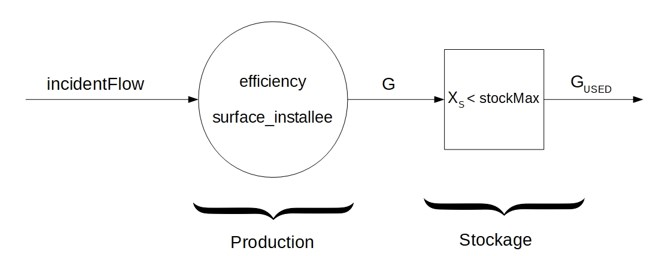
\includegraphics[width=0.75\textwidth]{figures/FeuilleFlux.jpg}
	\caption{text}
	\label{fig:FlowSheet}
\end{figure}

\subsubsection{Flow sheet parameters}

A flow sheet is initially defined by the set of limited parameters listed below (the values are given as an example):

\begin{itemize}
\item \textit{type : flow}

\item \textit{name : solar energy}

\item Incident flow ---  \textit{incidentFlow : 1e10}

\item Conversion efficienc ---  \textit{eff\_init : 0.15}

\item Installed surface ---  \textit{surface\_installee : 1e-9}

\item Usable as energy ---  \textit{isEnergy : True }

\item Maximum storage capacity ---  \textit{stockMax\_init : 50}
\end{itemize}

\subsection{Structure of the physical core}

The physical core is the place where manufactured goods are made. The structure diagram of how this area works is shown in the figure~\ref{fig:kernel}.

\begin{figure}[h]
	\centering 
	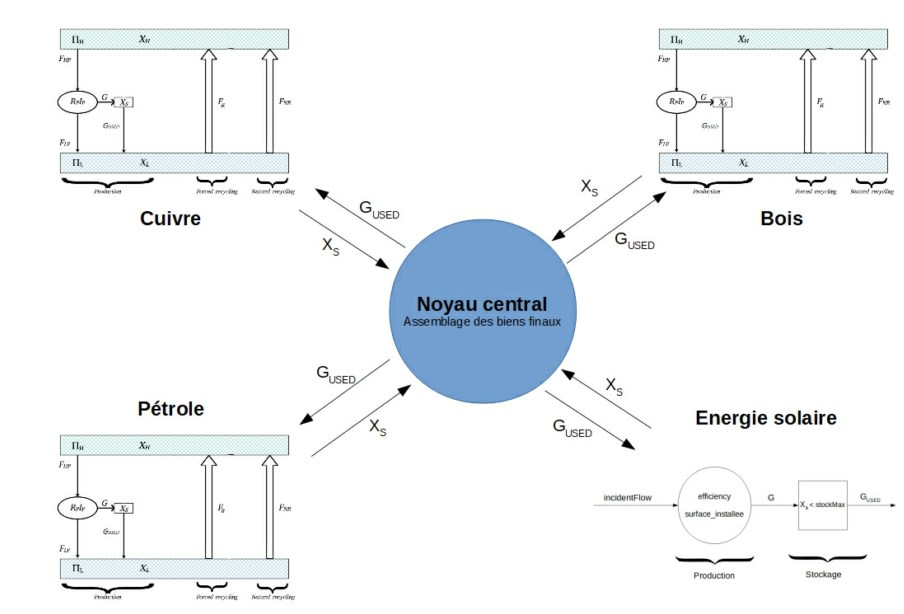
\includegraphics[width=0.75\textwidth]{figures/NoyauCentral.jpg}
	\caption{text}
	\label{fig:kernel}
\end{figure}

The ``recipes'' for the production of manufactured goods are indicated in the sheet \textit{world.txt}. The \textit{main.py} program carries out automatically the realization in respect of these ``recipes''.

\subsection{Structure of the economic zone}

The economic zone is the place where the economic model is coded. To illustrate this point, two examples are given~:

\begin{enumerate}
\item Goodwin

\item Sollow
\end{enumerate}

The advanced user can build his own model following the general structure of an economic structure of an economic sheet (see Appendix~A)







\section{Simulate with \ed}

\subsection{List of files}

You must have in a folder:

\begin{itemize}
	\item the python scripts :
	
	\begin{itemize}
		\item the file \textbf{PhysicalWorld.py}
		
		\item a file describing your economic sphere. In this manual we will use the Goodwin model, described in \textbf{Goodwin.py}.
		
		\item the file \textbf{main.py}
	\end{itemize}
\end{itemize}

\begin{itemize}
	\item as many parameterization files as necessary. At least one resource sheet must be used.
	
	\begin{itemize}
		\item \textbf{world.txt} (required)
		
		\item \textbf{oil.txt} if you have an oil sheet
		
		\item \textbf{copper.txt} if you have a copper sheet
		
	\end{itemize}
\end{itemize}

The file \textbf{main.py} can then be run to launche the simulation. The time step \textit{deltat}, and the temporal extent of the simulation \textit{tmax} can be mofied in \textbf{main.py}.

\subsection{Physical sphere settings}

To modify the physical parameters (cell parameters, and global parameters of the physical sphere), it is necessary to modify the \textbf{*.txt} files.

\subsubsection{Add a cell}

Parameter setting of the new cell:
\begin{enumerate}
	\item to create a stock cell, take the template \textbf{StockCell.txt}, enter the desired parameters, and save under the name of the resource (\textit{e.g.} \textbf{copper.txt})
	
	\item To create a flow cell, do the same with the template \textbf{FlowCell.txt}
	
	\item then, add in \textbf{world.txt} your new cell in the \textit{cells} table.
	
	\item finally, add the column corresponding to recipeMatrix in \textbf{world.txt}
\end{enumerate}

\subsubsection{Retract a cell}

\begin{enumerate}
	\item Delete the cell in the cells table in \textbf{world.txt}
	
	\item Delete the corresponding column from recipeMatrix in \textbf{world.txt}
\end{enumerate}

\subsubsection{Modification of the parameters and initial values of the variables of the physical sphere}

\begin{itemize}
	\item The global parameters and initial values of the global variables of the physical sphere are stored in the \textbf{world.txt} files.
	
	\item The parameters and initial values of the variables of the sheets are stored in the files \textbf{Name-Of-The-Sheet.txt}.
	
	\item Don't forget to save the file \textbf{*.txt} after modifying a value.\footnote{Caution, reading the parameters in the files is {unstable}. You must be careful to respect the spacing, not to add a line break at the end, etc. In particular, the strings in the cell array (e.g. ``~copper.txt~'') are then used to redirect to the file ``~copper.txt~'' for the initialization of the copper sheet. The name of the file containing the parameters of the sheet must therefore be the same string as the one that appears in cell.}
	
	\item The message \texttt{"~world successfully created~"} is printed when the model has been initialized.
\end{itemize}


\subsection{Setting up the economic zone: the Goodwin case}
We show figure~\ref{fig:SetGoodwinParameters} an example of \textit{goodwin.txt} file that set the parameters of the Goodwin economic model.

\begin{figure}[h]
	\centering
	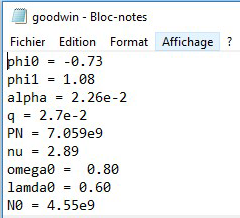
\includegraphics[width=0.3\textwidth]{figures/Goodwin-txt.png}
	\caption{text}
	\label{fig:SetGoodwinParameters}
\end{figure}

\begin{itemize}
	\item $phi0$ and $phi1$ are the parameters of the Philipps curve
	
	\item $alpha$ is the growth rate of labor productivity
	
	\item $q$ is the growth rate of the population
	
	\item $P_{N}$ is the maximum value of the population (the real growth rate of the population $N$ is $q \, (1-N/P_{N}))$)
	
	\item $nu$ is the productivity of capital
	
	\item $omega0$, $lambda0$ and $N_{0}$ are the initial values of the wageshare,
	employment rate and population
\end{itemize}


\section{Elementary case study}

\subsection{Parametrization}

We propose to illustrate the functioning of \ed\ by a case study based on the following:

\begin{itemize}
\item Four resources. Two are material, (copper \textit{Co} and wood \textit{Wo}), and two are energies (oil \textit{Oi} and solar energy \textit{So})

\item  Recipes are build on energy conservation. Three recipes for three different goods are considered~:

	\begin{itemize}
	\item Good 0  can be obtained with 1 unit of copper and 2 units of energy,  
	
	\item Good 1 can be obtained with 1 unit of copper and 2 units of wood and 3 units of energy
	
	\item Good 3 (copper recycling) can be obtained with 1 unit of energy 
	\end{itemize}

\item Target energy mix Mix énergétique cible, is composed of 90\% solar and 10\% oil.
\end{itemize}

\begin{figure}[h]
	\centering
	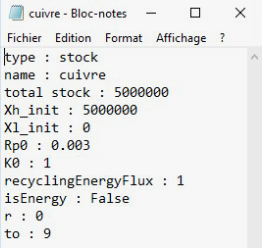
\includegraphics[width=0.3\textwidth]{figures/param_copper.png}
	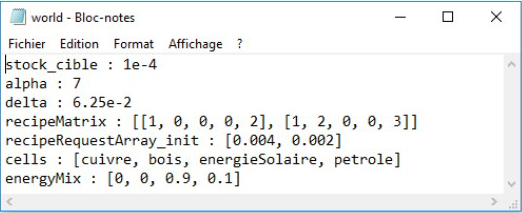
\includegraphics[width=0.65\textwidth]{figures/param_world.png}
	\caption{text}
	\label{fig:parametrization}
\end{figure}

\noindent Screenshots of \textbf{world.txt} and \textbf{copper.txt} parametrization are shown in figure~\ref{fig:parametrization}. In the main file \textbf{main.py}, the following parameters (see figure~\ref{fig:MainParametrization}) must be set~:

\begin{enumerate}
	\item Economic model. Here \textit{Solow}, parameterized by the correspondinf file \textbf{solow.txt} 
	 
	
	\item Time step and the duration of the simulation
\end{enumerate}

\begin{figure}[h]
	\centering
	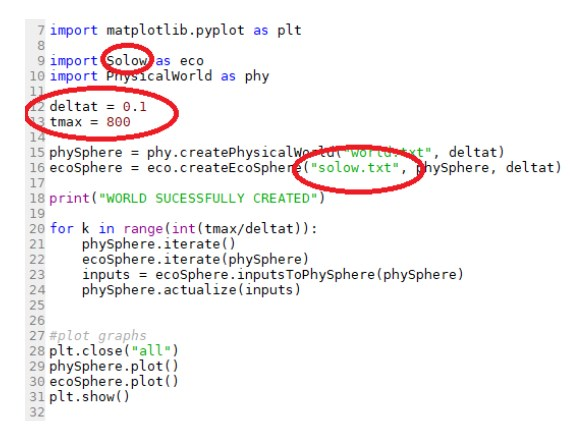
\includegraphics[width=0.5\textwidth]{figures/Parametrisation2.jpg}
	\caption{text}
	\label{fig:MainParametrization}
\end{figure}

%\begin{figure}[h]
%\centering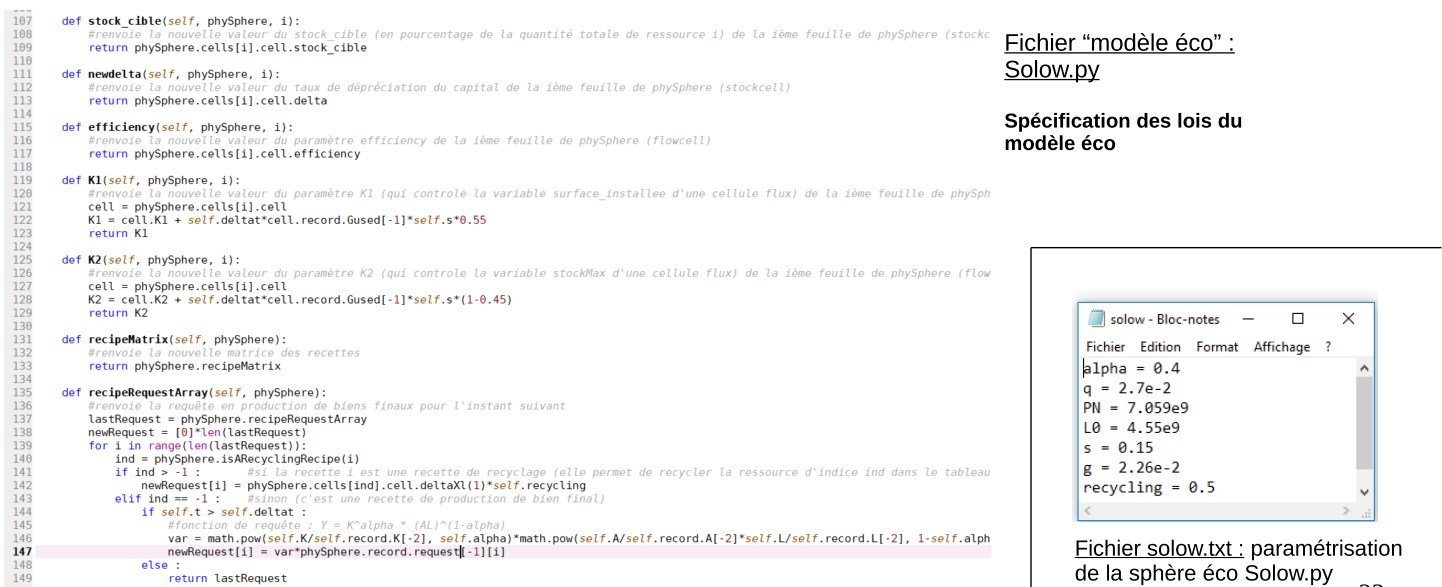
\includegraphics[width=0.95\textwidth]{figures/Parametrisation3.jpg}
%\end{figure}

\subsection{Results}

Running the simulation via the module \textbf{main.py} leads to the results shown in figure~\ref{fig:ResSimulProd} for production and energy. All the information related to each sheet being recorded, it is then possible to follow the specific evolution of their parameters, for example see in figure~\ref{fig:ResSimulOil} for oil.



\begin{figure}[h]
	\centering
	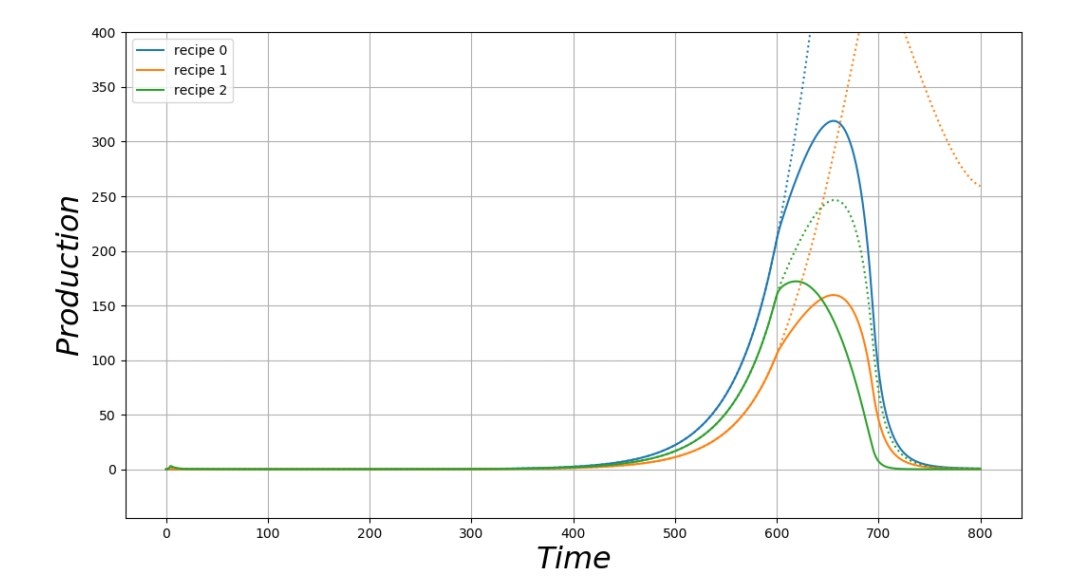
\includegraphics[width=0.45\textwidth]{figures/ResultatSimul.jpg}
	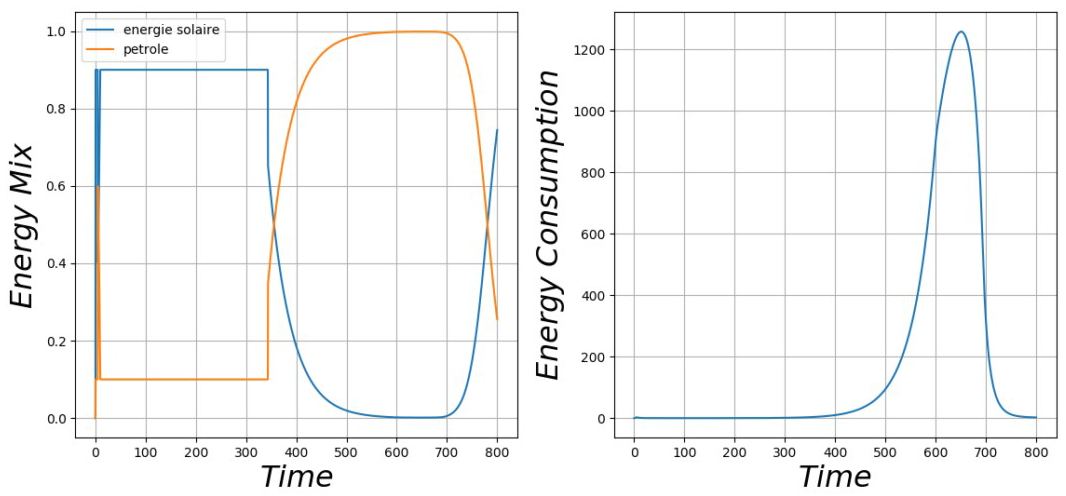
\includegraphics[width=0.51\textwidth]{figures/ResultatSimulE.png}
	\caption{text}
	\label{fig:ResSimulProd}
\end{figure}



\begin{figure}[h]
	\centering
	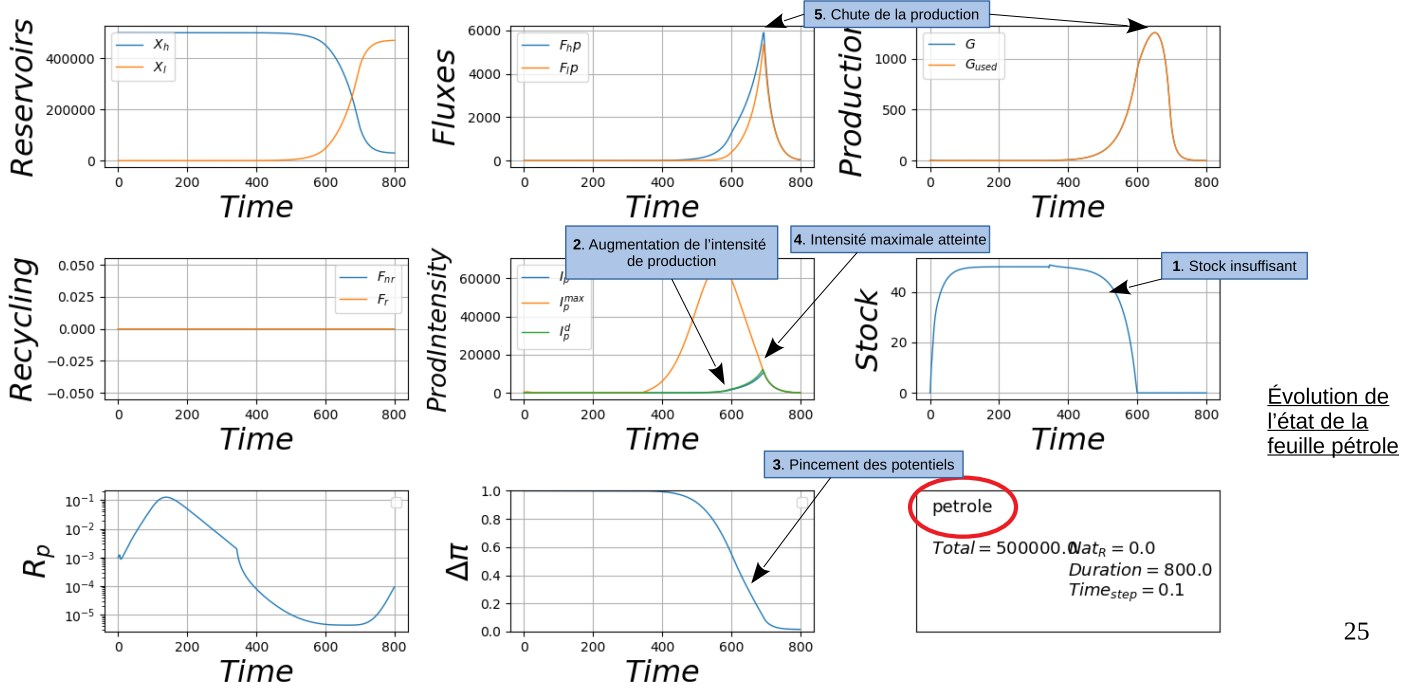
\includegraphics[width=0.9\textwidth]{figures/ResultatSimulPet.jpg}
	\caption{text}
	\label{fig:ResSimulOil}
\end{figure}


\begin{appendix}
	\section{How to use an alternative business model~?}
\subsection{Use another economic model among the available models library} 
If we wish to use a different economic model for the economic sphere, among the available models, we must make the following modifications in the main.py file 
\begin{itemize} 
	\item Line 9~: Specify the name of the . py file describing the eco-sphere (here Goodwin.py) 
	\item Line 17-18~: create an instance of the eco-sphere with a call to the eco.createEcosphere() function - check that the arguments taken by this function correspond to the arguments requested by the createEcoSphere function in your EcoModel. py file (here Goodwin.py) 
	\item Line 36: In the same way, check the arguments taken by the ecoSphere.inv() function 
	\item Line 40: In the same way, check the arguments taken by the ecoSphere.iterate() function 
	\item Line 42: In the same way, check the arguments taken by the ecoSphere. newProdRequest() 
\end{itemize} 
\begin{figure}[h] 
	\centering 
	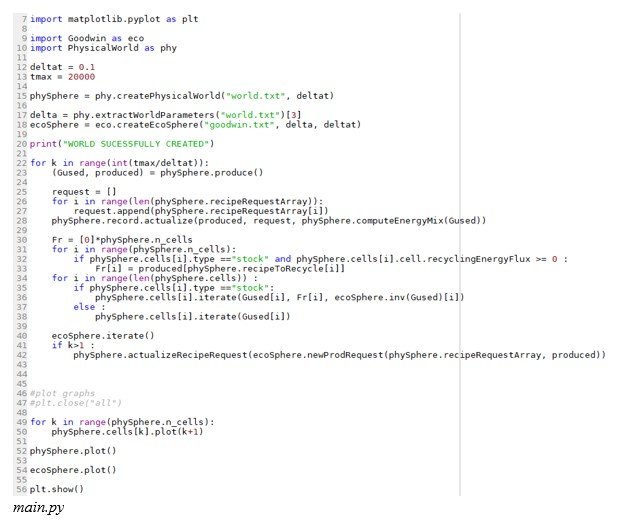
\includegraphics[width=1.0\textwidth]{figures/Main-py.jpg} 
\end{figure} 

\subsection{Create a new eco-model} 
It is possible to insert any eco-model into the DyCoEco program. If you want to write one yourself to add it to the library of available models, you must respect the following structure in your script~: The .py file must contain :  
\begin{itemize} 
	\item a function createEcoSphere 
\end{itemize} 
\begin{itemize} 
	\item a class EcoSphere containing:  
	\begin{itemize} 
		\item a constructor 
		\begin{verbatim}
			\_init\___ 
		\end{verbatim}
		\item a function iterate 
		\item a function inv 
		\item a function newProdRequest 
		\item a function plot 
	\end{itemize} 
\end{itemize} 
An example of economic model (trivial) respecting this structure is given below (ecoVide. py).\newline The role of the above mentioned functions is also detailed \begin{figure}[h] 
	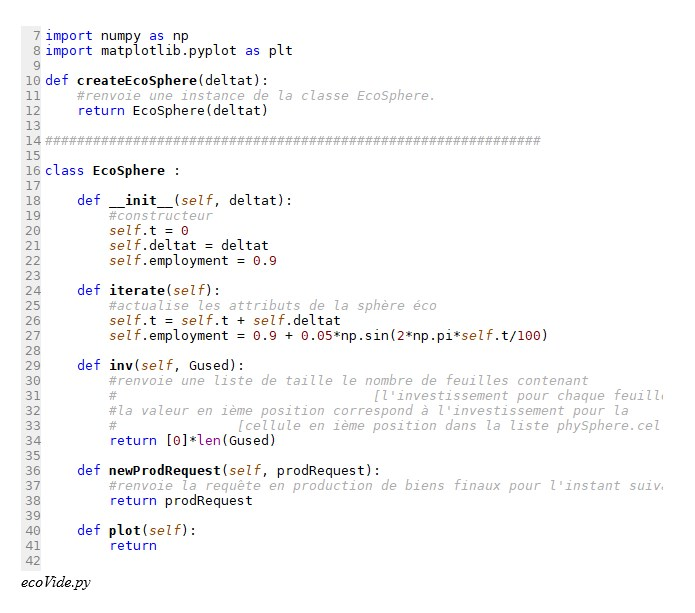
\includegraphics[width=1.0\textwidth]{figures/EcoVide-py.jpg}
\end{figure}  

\section{Equations governing a stock sheet}  
\subsection{General architecture} 
Resources of type "~stock~" are assumed to be in constant global quantity. A unit of resource "~stock~" can be in three different states.  It can be "\textit{available}~", i.e. it can be extracted by the production apparatus for further processing (recoverable resources). It can also have already been extracted, and be \textit{waiting} for transformation into final good. Finally, it may be ÒusedÓ, i.e. the economic sphere is unable to valorize it.  

We define three reservoirs containing the resources in each of these three states: a high reservoir for the available fraction of the resource, a stock for the fraction of the resource awaiting further transformation, and a low reservoir for the used fraction of the resource.  

We note $X_{H},X_{S}$ and $X_{L}$ the corresponding quantities, and $X_{T}$ the total quantity of resource.  Thus, we have at each instant:
\begin{align}
	X_{H}+X_{S}+X_{L}&=X_{T}
\end{align} 
Then, we strictly count the movements between these three reservoirs.  Resource extraction is the process of converting a unit of "~available~" resource to a unit of "~pending~" resource. This process is usually not 100\% efficient: a fraction of the extracted available resource is immediately transformed into waste. This process is analogous to the production of work by a heat engine: a certain amount of useful work W is produced from the difference in temperature between two thermostats, while a part of the energy coming from the hot source $Q_{C}$ is dissipated as heat $Q_{F}$.  
\begin{figure}[h] 
	\centering 
	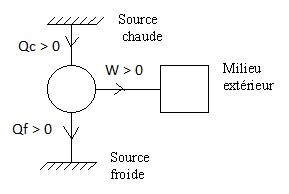
\includegraphics[width=0.6\textwidth]{figures/Carnot.jpg}
\end{figure} 
Here, the hot source becomes the "~available~" resource reservoir, the cold source the "~used~" resource reservoir, and the work produced is stored.  We note $F_{HP}$ the flow from the high reservoir, $F_{LP}$ the flow to the low reservoir, and $G$ the resource flow to the stock. Thus,
\begin{align}
	G & = F_{HP}-F_{LP}
\end{align} 
The resources in the stock $X_{S}$ are then transformed into the final good. After use, the resource becomes waste. We note $G_{USED}$ this flow between the stock and the low tank.  All these flows together define the production area. A used resource unit can sometimes be recycled. This recycling can be natural, or the consequence of a human activity. We note $F_{NR}$ the natural recycling flow, and $F_{R}$ the human recycling flow. 

\subsection{Production area}
As the available resource is exploited, its quality decreases, because the resource of good quality is exploited first. However, the quality of the resource has an impact on the effort required to extract it. For example, for a mining resource, it takes more effort (the intensity of production) after three years of exploitation than at the beginning of the exploitation to extract the same flow. In fact, the quality of the resource (its concentration in particular) has deteriorated. The notion of quality is therefore essential in the extraction process. Thermodynamics clearly establishes this distinction between quantity and quality. We therefore introduce here a notion of thermodynamics, the "potential". This is an intensive variable. The resources in the upper reservoir are at a certain level of potential, $\Pi_{H}$. $\Pi_{H}$ decreases as the resource is extracted from the upper reservoir. $\Pi_{H}$ is therefore an increasing function of $X_{H}$.  We have~: 
\begin{align}
	F_{HP} &= \Pi_{H} I_{P} \\
	\Pi_{H} &= f_1(X_H)
\end{align} 
The waste in the lower tank is a pollution, which has a negative feedback on production. This feedback is manifested by the increase in the potential of the low reservoir, 
\begin{align}
	F_{LP} &= \Pi_L I_P \\
	\Pi_{L} &= f_2(X_L)
\end{align}  
The choice of functions $f_{1}$ and $f_{2}$ is important if one wishes to obtain quantitative results with the model. If we only want qualitative results, we can just describe the form that these functions should have (increasing or decreasing, concave or convex, etc...)$_{.}$ In the following, we will take for $f_{1}$ an increasing and convex function, such that $f_{1}(X_{H}=0)=0,5$ and $f_{1}(X_{H}=X_{T})=1$. We will take for $f_{2}$ an increasing and concave function, such that $f_{1}(X_{L}=0)=0$ and $f_{1}(X_{L}=X_{T})=0.5$. 
\begin{figure}[h] 
	\centering 
	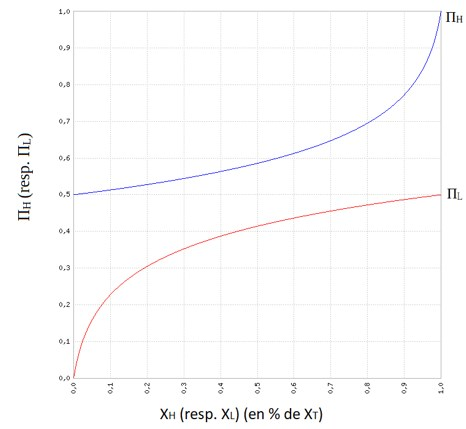
\includegraphics[width=1.0\textwidth]{figures/Potentiels.jpg}
\end{figure} 

When all of the resource is in the high reservoir, $\Pi_{H}=1$ and $\Pi _{L}=0$. The potential difference $\Delta \Pi$ is maximal. When all the resource is in the low tank, $\Pi_{H}=\Pi_{L}=0.5$. The potential difference is zero, and production is impossible. Economic activity without recycling leads to the passage of resources from the upper to the lower reservoir, thus a decrease in $\Delta Pi$. In other words, economic activity without recycling leads to a decrease in the subsequent capacity to produce.  Finally, extensive variables were introduced to describe the quantity $(X_{H},X_{L},X_{S},X_{T})$, and intensive variables to describe the quality of the resource $(\Pi_{H},\Pi_{L})$.
More precisely, producing at a high intensity is not equivalent to producing at a low intensity. At low intensity, the efficiency of the process is better, but the flow produced $G$ is less important. At high intensity, $G$ is higher but the yield is degraded.  We therefore introduce a \textit{resistance} $R_{P}$. We then have a friction term $R_{P}I_{P}^{2}$, and $F_{LP}$ becomes~:
\begin{align}
	F_{LP} &= \Pi_{L}I_{P}+R_{P}I_{P}^{2}
\end{align}
In summary, the equations describing the extraction are~: 
\begin{align} 
	F_{HP} & =\Pi_{H}I_{P} \\
	F_{LP} & =\Pi_{L}I_{P}+R_{P}I_{P}^{2} \\
	G & =F_{HP}-F_{LP}=\Delta \Pi I_{P}+R_{P}I_{P}^{2}
\end{align} 
The extracted flux $G$ is thus a function of the difference in potentials, of the production intensity, and of the resistance. Let's assume $\Delta \Pi$ and $R_{P}$ are fixed. G is then a parabolic function of $I_{P}$.  
\begin{figure}[h] 
	\centering 
	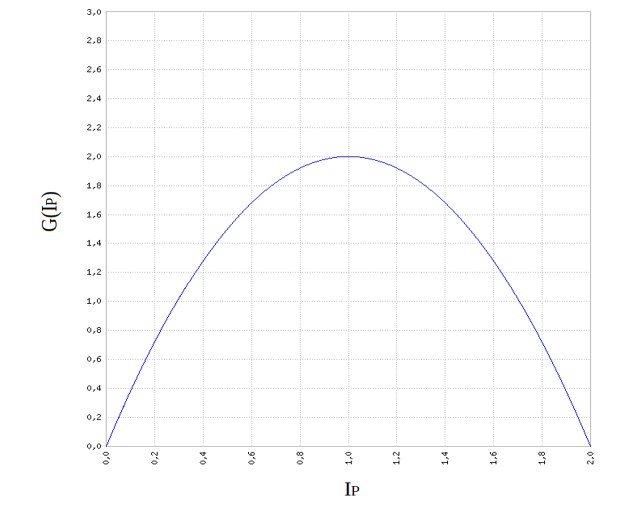
\includegraphics[width=1.0\textwidth]{figures/Prod-I.jpg}
\end{figure} 
The quadratic friction term implies that beyond a certain threshold $(I_{P}=\Delta\Pi/2R_{P})$, further increasing the production intensity actually decreases the extracted flux $G$. 

When we want to reach a certain level of extraction flow $G$, there are therefore zero, one, or two possible production intensities. If there are two, we will systematically choose the lower one. Thus, the value $(I_{P}=\Delta \Pi/2 R_{P})$, which allows the maximum extraction flow to be reached, is also the maximum value of $I_{P}$. We will note this value $I_{p}^{max}$.  Moreover, it is possible that the required extraction flow level $G$ is not achievable, depending on the pair $(\Delta \Pi ,R_{P})$. The maximum value of $G$ is 
\begin{align}
	[G^{max} &= \Delta\Pi^{2}/4R_{P}
\end{align}

It is therefore possible that the economic sphere sets a production demand that cannot be met. The possibility of such a production failure constitutes the heart of the model: it is here that the feedback of the physical sphere on the economic activity is manifested. Such a production failure is favored by~:  
\begin{itemize} 
	\item A high production request 
	\item A low potential difference (we speak of \textit{potential pinch}) 
	\item A high resistance 
\end{itemize} 
Moreover, the efficiency of the extraction process, defined by $\eta=G/F_{HP}$, is: \begin{align}
	\eta &= 1-\Pi_{L}/\Pi_{H}-R_{P}I_{P}^{2}/F_{HP}
\end{align} 
At zero intensity, we find an expression analogous to the Carnot efficiency. Then, the efficiency decreases as the intensity increases. It is thus necessary to find a compromise between efficiency $\eta$ and extracted flux $G$. Finally, the extraction process has a certain inertia. If we can instantly calculate the ideal production intensity to meet the demands of the economic sphere, the real production intensity adjusts with a certain delay. We define a \textit{requested production intensity }$I_{P}^{D}$. The delay is characterized by a \textit{characteristic production response time }$\tau$.  We then have 
\begin{align}
	dI_{P}/dt+tau I_{P} &= I_{P}^{D}
\end{align}
Note that this allows us to give a physical meaning to the model time. From now on, the period from $t=10$ to $t=20$ in the model, i.e. $\Delta t=10$, can be compared to the reaction times of the leaves, which have a physical meaning.  

\subsection{Recycling area}
The natural recycling flow is given by the relation: 
\begin{align}
	F_{NR} &= r\left( 1-\exp\left( \frac{X_{L}}{0.5X_{T}}\right) \right )
\end{align}
$r$ being the natural regeneration rate.  Sometimes, a process allowing to recycle a resource is known and mastered by the Man. This is called "human" recycling, as opposed to natural recycling. These human recycling processes are economic activities in their own right, and the recycling of a unit of resource requires an input of energy (and material). In the present state of the model, it is assumed that recycling "~humanly~" a unit of resource requires an input of \textit{x} units of energy. The value \textit{x} corresponds to the parameter \textbf{recyclingEnergy}, specific to each leaf. Not only is it necessary in general to have other resources than just energy to operate a recycling process, but the difficulty to recycle (i.e. the quantity of energy to bring to recycle a unit of resource) varies, according to the quality of the waste. This point will be improved in the further development of the model. We have introduced here a notion of finality of production~: the combination of certain resources allows the production of a good (here a service)~: the recycling of another resource. The notions of "final good" and "production revenue" formalize this idea. In the model, they are implemented at the level of the physical sphere, above the various resource sheets. We speak of a central core, encompassing all the resource sheets.  

\section{Equations governing a flux sheet}
 A "~flux~" type sheet is defined by an incident flux $P_{i}$ (integrated over the entire surface of the Earth), and a production apparatus characterized by a yield $\eta$ and an installed surface $S$ (in percentage of the Earth's surface). The production apparatus allows the extraction of this resource, \textit{ i.e.} its availability for further processing.  The extracted flux writes:
 \begin{align}
 	G &=\eta P_i S
 \end{align}
 This flux can be immediatly used or stored for further uses. The storage capacity is defined by the parameter $stock_{Max}$.  The use of the resource corresponds to a flow out of the stock, noted $G_{USED}$.  Thus, the stock $X_{S}$ verifies 
 \begin{align}
	 \Delta X_{S} 		& = G - G_{USED} \\
	   				0 & <X_{S}<stock_{Max}	
 \end{align}   

\section{Management of the central core coupling the physical sheets: ``recipes''}   
The central core is the zone of assembly of the resources previously extracted for formation of the final goods. The production recipes define the ingredients and quantities necessary to form a unit of a final good. For example, we can define the final good "~barque~" with the recipe~: 
\begin{align}
	5 wood + 3 energy &= 1 barque 
\end{align} 
The set of coefficients of the recipes defines a \textit{revenue matrix}, whose columns represent the resources and rows the final goods.  It is assumed that the demands of the economic sphere are expressed in units of final goods. The production demands of each resource are deduced from the coefficients of the revenues.  As the revenues define the proportions between the resources, the productions of each resource must adjust to each other permanently. For example, using the previous example, if wood production falls, energy production must fall by the same amount: there is no point in continuing to burn oil if we do not use the energy produced.  The implementation of strategies allowing to obtain this result has been the subject of several attempts. In a first attempt, the central core indicates (at each new time step) to each leaf the desired production level. The central core must therefore collect from the leaves the information concerning the quantities of resources available for use $(X_{S})$, process them, and then send back to each leaf the production level required for the next time step. The complexity of this process increases exponentially with the number of resources and the number of recipes. Finally, it was impossible to realize a satisfactory algorithm to process all these data, because such an algorithm requires the introduction of multiple conditional tests which make the process very unstable. Finally, it should be noted that this operation is not very natural (in a market system), since it corresponds to the hypothesis of a central regulating entity that indicates to each production sector the level of production required according to the results of the other sectors.  In the chosen strategy, a stock target is set for each sheet. Then, the production intensity of each leaf is adjusted in order to converge the value of the stock towards the target stock, and to maintain it there. More precisely, the variation of the requested production intensity $\Delta I_{P}^{D}$ is given by the equation~:
\begin{align}
	\Delta I_{P}^{D} &= a \, (X_s-X_s^{cible}) + b \, (\frac{dX_s}{dt}-0)
\end{align}
We want $X_S$ to converge to $X_s^{cible}$, and $\frac{dX_s}{dt}$ to 0.
$\Delta I_{P}^{D}$ is therefore a function of the gaps $X_{S}-X_{S}^{CIBLE}$ and $dX_{S}/dt-0$. At equilibrium, $\Delta I_{P}^{D}$ is zero. $a$ and $b$ are parameters defining the relative preference between the two objectives ($X_{S}=X_{S}^{CIBLE}$ and $dX_{S}/dt=0$).  
\begin{figure}[h] 
	\centering 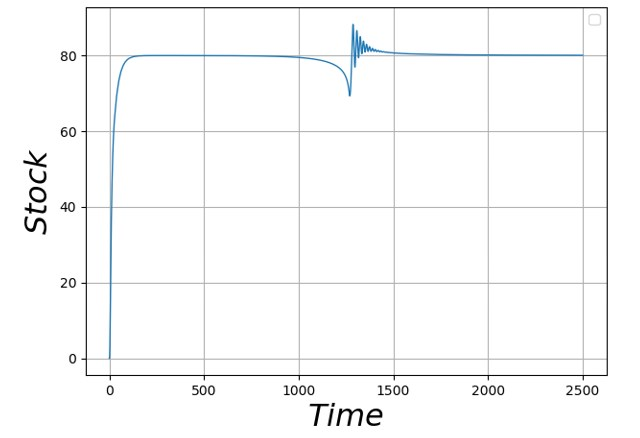
\includegraphics[width=1.0\textwidth]{figures/Stock-t.jpg}
\end{figure} 
In this strategy, each sheet sets its production intensity autonomously. We thus describe a situation where each production sector self-regulates its production according to what it sells. The introduction of the notion of recipe also makes it possible to bring out the idea that one cannot produce a final good without energy. Indeed, the production recipe indicates the quantity of energy needed to produce one unit of final good. If this quantity is not available, no final good is produced, i.e. the resource that has been extracted is not "used" in order to be transformed into a final good once it has been combined with energy. Faced with this non-use, and in order not to constitute too large a stock, the resource sheet will autonomously reduce its production intensity. Thus, the introduction of the notion of revenue makes it possible to retroact on the extraction of all resources in case of lack of energy~: nothing can be produced without energy. This reasoning is also valid in the case of a lack of production of a resource other than energy.  Thus, each leaf extracts a certain quantity of resources at each time step. It is added to the quantity of resources "in stock" $X_{S}$ available for further transformation. The determination of the number of units of final goods produced is a function:
\begin{itemize} 
	\item of the quantities of resources ``in stock'' 
	\item of the requests of production of final good coming from the economic sphere 
	\item of the matrix of receipts~ 
\end{itemize} 
It is thus a question of allocating the resources to the various receipts of production of final goods. There are various possible methods of allocation. For example~: to give absolute priority to the production of the final good $n^{o}1$ to the detriment of all the others, or, conversely, to produce final goods in equal quantities without taking into account the production requests, or again, to produce final goods by respecting as much as possible the proportions defined by the production requests emanating from the economic sphere.  This last strategy seems the most natural. It means that we consider that the production requests of final goods correspond to the market demand, and that we would like to satisfy all the requests simultaneously, but that in case of impossibility, we distribute the production default between all the final goods using this resource. The algorithm returns the resource allocations to the production of the different final goods.  

\subsection{Energy mix} 
When the production of a good requires energy, it can be realized whatever the origin of this energy: oil, coal, gas, nuclear, solar, etc. Therefore, the energy requirement must be specified in the recipe, not the requirement for each energy resource. This implies that we must indicate which of the leaves are energy resources. These resources are then used to meet the energy requirement. In this way, an effective energy mix is defined.  Furthermore, when launching a simulation, we define a desired energy mix, which we will try to satisfy when possible. The actual energy mix can be different from the desired energy mix, for example if an energy resource is missing.  Finally, the physical sphere describes the evolution of the state of the resource over time, and accounts for the material and energy flows generated by the production of goods and by recycling. But the desired levels of production and recycling are human decisions, to which the physical sphere only responds. The laws describing the evolution of these demands are described in the economic sphere. 

\section{Economy}
\subsection{Economic sphere} 
\subsubsection{{General structure}}  
The role of the economic sphere is to specify the evolution of all economic variables. In particular, it indicates to the physical sphere~:  
\begin{itemize} 
	\item production requests for each final good 
	\item a ``human'' recycling request for each concerned resource 
	\item the desired energy mix 
	\item the investment, for each sector (leaf), which allows to increase the capital. The capital is directly linked to the resistance R$_{P}$ of the ``stock'' leaves, and to the variables \textit{installed surface} S and stockMax of the ``flow'' leaves 
	\item the level of target stock for the ``stock'' leaves 
\end{itemize} 

\subsection{{technical progress}}  
We specify in the economic sphere the laws describing the possible technical progress. The technical progress corresponds here to the decrease of the quantities of resources necessary to the production of a unit of final good. It is therefore a gain in efficiency: it takes less energy to machine a part, or less aluminum to produce a can. In the model, this corresponds to the decrease in the coefficients of the revenue matrix. Another form of technological progress is the discovery of a new material, or the development of a technology to substitute one material for another. For example, in the 1970s, demand for nickel fell by 20 percent, mainly because of the substitution of manganese for nickel in the production of automobile bumpers. In the further development of the model, the notion of substitution can be represented by a change in production revenues. Let us note that the economic sphere only addresses "production requests" to the physical sphere. This implies that these requests can be, or not, satisfied, for example in case of pinching of the potentials describing the state of the resource. This point is crucial, since it implies the possibility of a feedback from the physical sphere to the economic sphere. The set of laws describing the evolution of these variables constitutes the economic sphere. The architecture of the model code makes these laws easily accessible and modifiable. In the project approach, the user is encouraged to test various parameters, laws and macroeconomic models. A library of examples of such laws is being built up. In particular, one can use the production functions of macroeconomic models as a production request, and the investment described by these same models as an investment.  

\subsection{Levels of use of the model}
There are several levels of use of the model. The first level consists in making the model run by using in the economic sphere laws already pre-written and by varying only the parameters (number of resources, their characteristics, choice of the energy mix, required recycling, etc). For example, to vary the growth rate of labor productivity in a Solow model.  The second level consists of testing various laws (and macro-economic models) among the library of laws available. This allows us to observe the sensitivity of the physical sphere to the choice of these laws.  Finally, the user who already knows the model well is invited to propose new laws himself, in order to enrich the library. A law can correspond for example to the production function of a macroeconomic model, to an assumption concerning the rhythm of technical progress, or to the introduction of a feedback between the state of the resources and the desired energy mix.

\subsubsection{{Example model: Solow}} 
{An example of an economic sphere based on the Solow model}  
\begin{figure}[h] 
	\centering 
	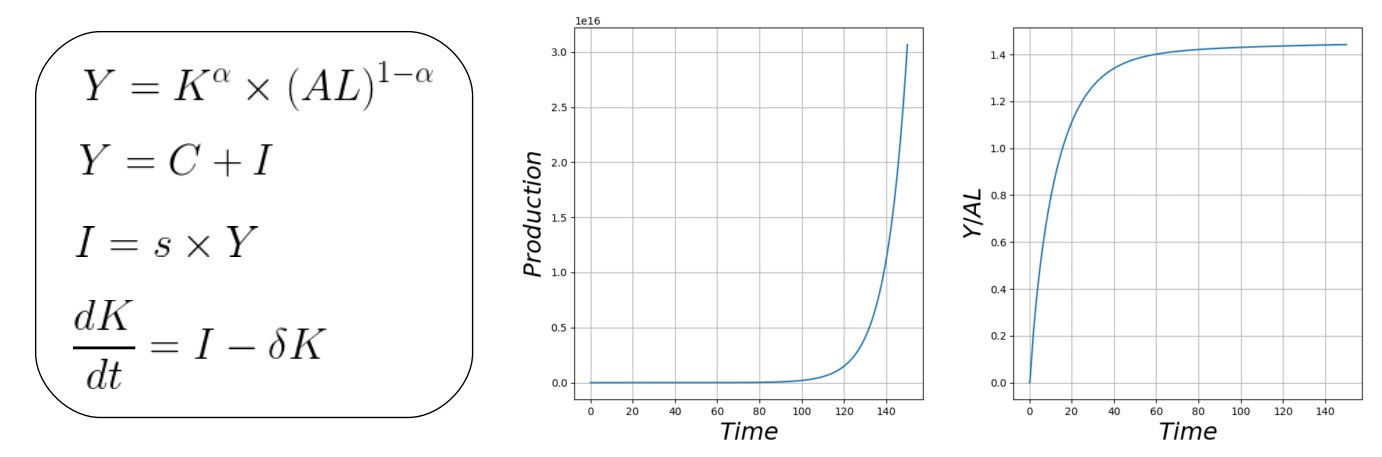
\includegraphics[width=1.0\textwidth]{figures/solow2.jpg}
\end{figure} 
The Solow model, created in 1956, is a macroeconomic model that explains growth by the accumulation of capital, the growth of the active population, and the growth of labor productivity. It is a reference model of neo-classical economics.  It uses a two-factor Cobb-Douglas production function:
\begin{align}
	Y=K^{\alpha}(AL)^{1-\alpha}
\end{align}  with :  
\begin{itemize} 
	\item $Y$ the production 
	\item $K$ the capital 
	\item $A$ the labor productivity 
	\item $L$ the active population 
\end{itemize} 
The labor productivity increases exogenously, at rate $g_{A }$.  The active population also increases exogenously. In our model, we choose to make the active population tend towards a limit value $P_{L}$: the growth rate of the active population is $g_{L}=q(1-L/P_{L})$. The growth rate decreases as the labor force L approaches its limit value P$_{L}$.  Capital erodes at the rate $\delta K$, an erosion compensated by investment $I$.  
\begin{align}
	\frac{d K}{d t} & = I \, \delta \, K
\end{align} 
A part $s$ of the production is reinvested:  
\begin{align}
	I &= s \, Y 
\end{align}
In this model, the output $Y$ increases exponentially, thanks to the growth of labor productivity. The output per unit of actual work $Y/AL$ converges to a stationary state.  

\subsection{Adaptation for the economic sphere}
\subsubsection{Production request function}
We use the production function of the Solow model as the production query function (section 1.2.1).  We initialize the production queries for each final good at the start of the simulation. At each time, we compute the query for time $t+dt$ from the production result of time $t$
\begin{align}
	 Y_{REQ}(t+dt) &= Y(t)\ast\left( \frac{K(t+dt)}{K(t)}\right) ^{alpha}\left( \frac{A(t+dt)L(t+dt)}{A(t)L(t)}\right) ^{1- \alpha}%]
\end{align}
with 
\begin{itemize} 
	\item $Y_{REQ}$ the production request addressed to the physical sphere.  
	\item $Y$ the actual production (which may differ from the production request) 
\end{itemize} 
Thus, as long as the production request is satisfied, the production is equal to that predicted by the Solow model. If the production request is not satisfied at time t, the request at time t+dt adapts: we do not continue to ask for exponential growth indefinitely when actual production no longer follows.  

\subsubsection{Investment}
The investment is defined for each resource sheet. We define a parameter s common to all the leaves, which corresponds to the fraction of the reinvested production. The production of each leaf corresponds to what was effectively used by the central core of the physical sphere, \textit{i.e.} the variable $G_{USED}$.  Thus, 
\begin{align}
	I &= s\, G_{USED}
\end{align}

\subsubsection{Recycling query} 
For the recycling query, we define the following law: we wish to recycle a constant proportion of the quantity of waste produced We define this proportion at the initialization of the simulation, by indicating the value of the recycling parameter between 0 and 1. The equation of the recycling request is thus:
\begin{align}
	Y_{REQ}(t+dt) &= (F_{LP}(t)+G_{USED}(t))\ast recycling
\end{align}
This law is only a proposal. One could also consider the total amount of waste $X_{L}$ for the recycling query, not just the change in that amount.  

\subsubsection{Other Economic input}
It was chosen not to vary the target level of stock requested from the leaves, nor the desired energy mix, nor the quantities of resources needed to produce one unit of each final good (coefficients in the revenue matrix). The model has been created with the aim of allowing the user to propose and test his own functions and scenarios of variation of all these requests from the economic to the physical sphere. Thus, the part containing all the functions accessible to the user is located in a separate, short and commented file.  	

\subsection{Analysis} 
The purpose of this model is not to reproduce as faithfully as possible the trajectory of the world economy over the last few decades, nor to predict quantitatively what might happen. It is a tool for testing a multitude of hypotheses, scenarios and macroeconomic models in a framework that explicitly takes into account the impact of economic activity on the physical sphere and its feedbacks.  The number of hypotheses and scenarios that can be tested is limited only by the imagination of the user. Therefore, this section does not aim at delivering a complete analysis of what can be derived from the model, but at delivering some fundamental results obtained. We will try to present these results, and then illustrate them with an example that allows us to isolate the phenomenon or reason discussed.  We find results that are expected but not obtained by most macroeconomic models. This allows us to verify that this tool achieves its objective of proposing a physical basis for macroeconomic models by directly taking into account the flows of matter and energy generated by economic activity. 

\section{Physical-Economic Feedback Mechanism}
\subsection{Feedbacks from the physical sphere on economic activity} 
One observes, according to the parameterization of the situation, feedbacks from the physical sphere on the economic activity. In particular, when the recycling flow (natural or human) is zero (non-recyclable resources for example) or insufficient, we observe the depletion of "stock" resources, and their feedback on production. This feedback takes the form of slope breaks: it is therefore more a question of collapse than of progressive decrease. Let us illustrate this point with a toy example that allows us to see the mechanism of the collapse.  We consider a world with three resources, copper, wood and oil. These three resources allow us to produce two final goods, according to the recipes:  
\begin{itemize}
	\item copper + energy = good 0
	\item copper + wood + energy = good 1
\end{itemize} 
For simplicity, we consider that we are not able to recycle copper (or that we do not wish to). Wood is naturally recycled. We also assume that the resistance of the production equipment is constant (zero capital erosion and zero investment). Finally, we place ourselves in a zero growth scenario. The demand for final goods is constant (respectively 12 good 0 and 18 good 1 per time unit).  
\begin{figure}[h] 
	\centering 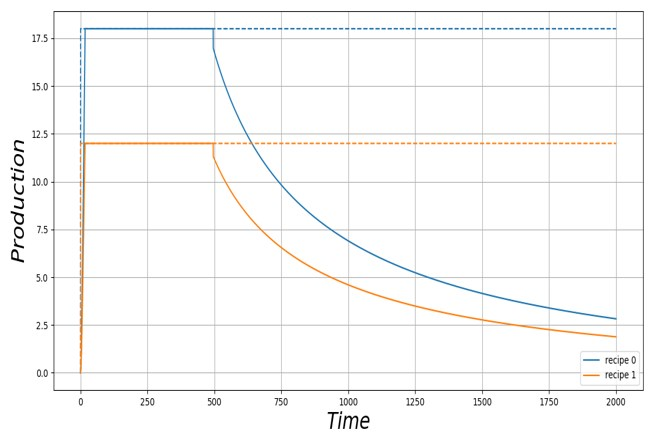
\includegraphics[width=1.0\textwidth]{figures/Production7.jpg}
\end{figure} 
We observe a fall in the production of goods 1 and 2 at t=500, despite a constant demand for production. The production seems to converge exponentially towards zero production (which is confirmed by a logarithmic scaling).  The copper and oil resources (the only energy resource in the simulation) are common to both production recipes. The simultaneity of the falls in production of goods 0 and 1 suggests that one of these two resources has failed.  
\begin{figure}[h]
	\centering 
	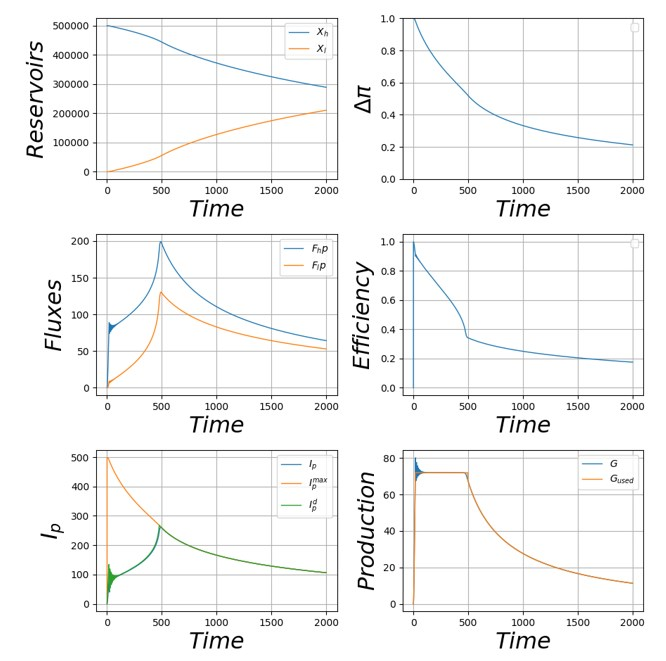
\includegraphics[width=1.0\textwidth]{figures/Tableau-Bord8.jpg}
\end{figure} 
Indeed, the state of the oil resource seems to have deteriorated rapidly, leading to a drop in oil production at t=500. Let's examine the mechanism leading to this collapse.  Figure 8a shows that the upper reservoir is gradually emptying, while the lower reservoir is filling. As a result, the potential difference decreases (Figure 8b). Despite a constant production demand, the oil flows from the upper reservoir (FHP) to the lower reservoir (FLP) increase rapidly, due to the pinching of potentials (Figure 8c). At the same time, the efficiency of the process drops (Figure 8d). The production intensity increases to compensate for the drop in efficiency and satisfy the demand. The maximum possible production intensity decreases, and at t=500, the production intensity reaches the maximum production intensity (Figure 8e). Immediately, output falls (Figure 8f).  Thus, a zero growth scenario, without recycling, leads to a runaway with an explosion of resource flows to compensate for the loss of efficiency, in a vicious circle. We observe here a production failure linked to the exhaustion of a non-renewable and non-substituted resource.  
\subsection{Stable state}
However, a stable economic activity (which does not collapse in infinite time) is possible, if it involves the use of only recyclable stock resources (naturally or humanly) and renewable resources (flow resources).  To illustrate this point, we place ourselves in a situation similar to the previous example, replacing the "oil" sheet by a "solar energy" sheet. The demand for final goods 0 and 1 is constant. We assume that the wood resource is very abundant, contrary to the copper resource. However, we are able to recycle copper, by means of an energy input: one unit of energy allows to recycle one unit of copper.  It is also assumed that the installed surface of solar panels is very large, and that there is no erosion of capital. Thus, the amount of renewable energy is far greater than the needs of the economic activity. This is a strong assumption.  From $t=0$ to $t=500$, we decide not to recycle the copper. $At=500$ and for all subsequent instants, we decide to recycle 100\% of the newly produced copper waste.  The system seems stable (Fig. 9). But the observation of the evolution of the state of the copper resource shows that the decision to set a recycling demand of 100\% at t=500 has allowed to avoid a collapse, and to reach this stable state (Fig. \ref{Fig10}).  
\begin{figure}[h] 
	\centering 
	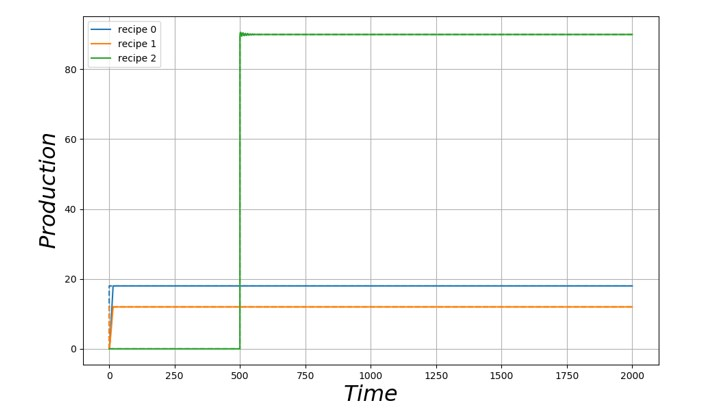
\includegraphics[width=1.0\textwidth]{figures/Production9.jpg}
	\label{Fig9}
\end{figure} 
\begin{figure}[h] 
	\centering 
	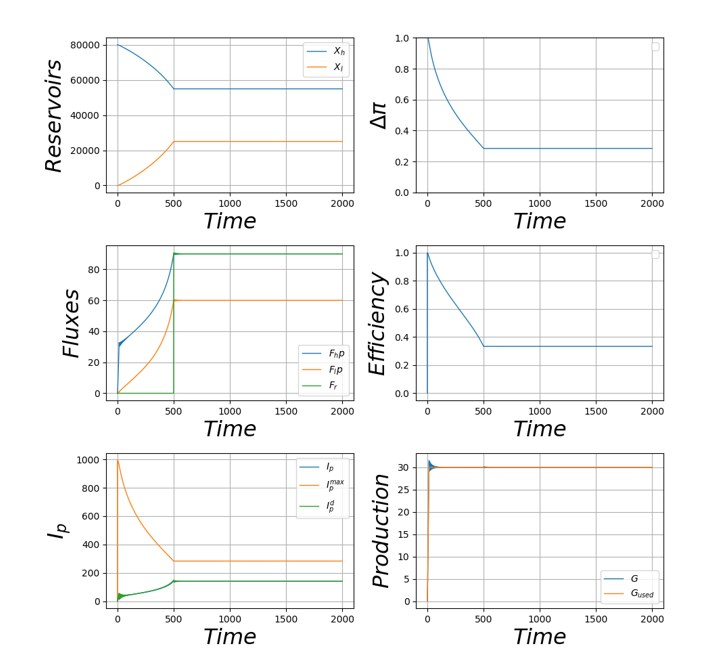
\includegraphics[width=1.0\textwidth]{figures/Tableau-Bord10.jpg}
	\label{Fig10}
\end{figure} 

\subsection{Shift from an economy based on flow resources to an economy based on stock resources} 
There is thus, for a given set of resources and revenues, a maximum stable level of production. The economic activity can exceed this maximum stable level thanks to the use of "stock" resources whose exploitation rate is virtually unlimited. But if the exploitation of these resources is faster than natural recycling, or if it is not accompanied by an equal increase in human recycling (especially if this is impossible, as with fossil resources), there is a risk of degrading these resources, so that the new state is not stable.  In the end, the limiting factors are :  
\begin{itemize}
	\item the use of stock resources which one does not know how to recycle, and for which one does not find substitutes.  
	\item The production of renewable energy, necessary for the recycling of all the other stock resources. 
\end{itemize} If the stock resources are depleted, we forcibly return to a stable level, verifying the conditions stated previously (section 2.2). The degradation of the state of the stock resources that has occurred is irreversible, and the new maximum stable production level has decreased.  To illustrate this, we consider a world with four resources: copper, wood, oil and solar energy. For the sake of simplicity, we again assume that we cannot recycle copper, but that this resource is extremely abundant. It is also assumed that the regeneration rate of wood is very high.  We consider the same revenues as before (section 2.1). The production demand of the final goods follows an exponential growth trajectory obtained by a `Solow' type law, similar to the one described in section 1.2.2. The initial production demands are close to zero.  The desired energy mix is: 100\% solar energy. The actual energy mix may be different, if the desired energy mix does not meet the production requests.  
\begin{figure}[h] 
	\centering 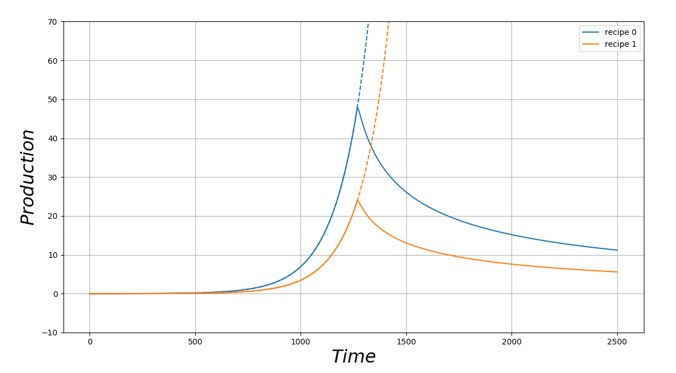
\includegraphics[width=1.0\textwidth]{figures/Production11.jpg}
	\label{Fig11}
\end{figure} 
We observe (Fig. \ref{Fig11}) in a first step an exponential increase of the production of goods 1 and 2, following the exponential growth of the production requests. At t=1250, the production of goods 1 and 2 falls, and the production requests are no longer satisfied. The production flows seem to converge to a lower but non-zero level.  
\begin{figure}[h] 
	\centering 
	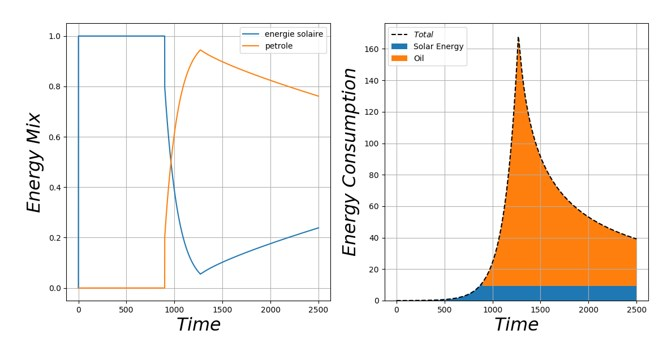
\includegraphics[width=1.0\textwidth]{figures/Energie12.jpg}
\label{Fig12}
\end{figure} 
The study of the evolution of the real energy mix over time indicates that at first ($t<800$), the energy need is entirely covered by the "solar energy" sheet (Fig. \ref{Fig12}). The actual energy mix is thus equal to the desired energy mix. For $t>800$, the energy need exceeds the solar energy production. We therefore call upon the oil sheet in order to continue to satisfy the energy demand. The real energy mix sees the place of oil becoming preponderant, as the energy demand grows. The oil sheet thus allows to continue to follow the exponential growth trajectory beyond the level allowed by the sole use of solar energy. At t=1250, oil production drops, suggesting a production failure of the leaf. A look at the evolution of the state of the oil sheet confirms this. The production of final goods falls, following the production of oil. The energy mix is gradually returning to a 100\% solar mix. The production levels converge towards the maximum level allowed by the available solar energy flow. 
 
\subsection{change in capital} 
All the illustrations so far come from simulations with fixed capital: the rate of capital erosion was zero, and so was the investment. Thus, the resistances $R_{P}$ of the stock sheets and the "installed area" parameters of the flow sheets were constant. The introduction of an erosion rate and a non-zero investment modifies the observed trajectories.  In the following, it is assumed that investment in the capital of a leaf is a fixed proportion of the production of that leaf: the sector "sells" x units of resource, and reinvests a proportion s. This is the investment law described in section 1.2.2.2. Note that the results presented below depend heavily on this investment law. In particular, it would be sensible to write a law modeling a situation where sector A can choose to invest a share of its revenues in sector B if it is more "profitable". The whole approach of the project consists in leaving the economic modeling part accessible to the user in order to allow him, for example, to test such a law.  The notions of capital erosion and investment lead to the appearance of virtuous and vicious circles in a context of increasing production demand.  As long as production increases, investment increases. Capital therefore increases as well, and the RP resistance decreases. The friction term therefore decreases, and the maximum value of the produced flow GMAX increases. Production can therefore increase even more, and so on.  Conversely, if production falls, investment falls, and so does capital, and resistance increases, which further aggravates the fall in production.  To illustrate this, we consider a world with three resources: copper, wood, oil, and two revenues (the same as above). Copper and wood are assumed to be very abundant. The production request is exponentially increasing. We carry out two successive simulations, one with zero capital erosion and investment, a second with positive capital erosion and investment (Fig. \ref{Fig13}).  
\begin{figure}[h] 
	\centering 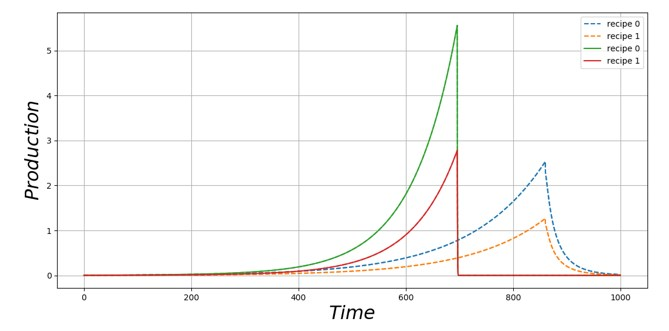
\includegraphics[width=1.0\textwidth]{figures/Production13.jpg}
	\label{Fig13}
\end{figure}
We can see that the growth and decay are much faster in the simulation with investment and capital erosion. This can be explained by looking at the evolution of the state of the oil sheet.  
\begin{figure}[h] 
	\centering 
	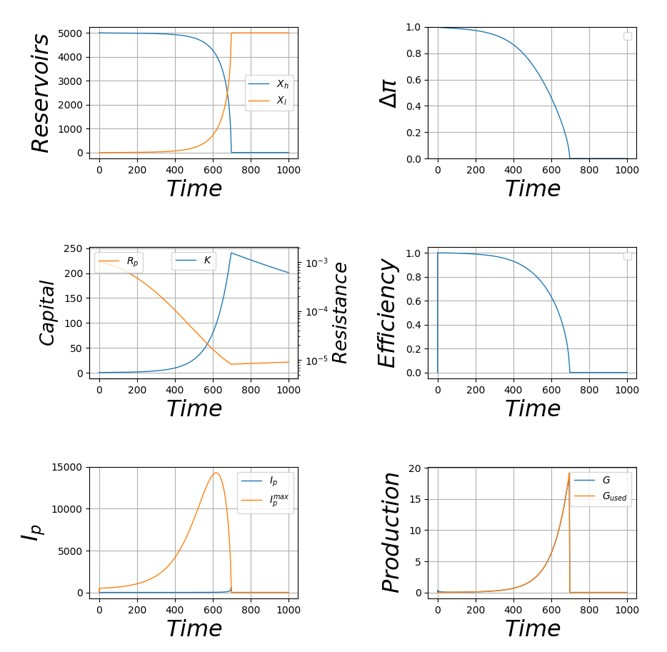
\includegraphics[width=1.0\textwidth]{figures/Tableau-Bord14.jpg}
	\label{Fig14}
\end{figure} From t=0 to t=700, oil production increases, in response to the exponential increase in demand. As a result, investment increases, which increases capital and decreases resistance (Fig. \ref{Fig14}c). As a result, the maximum possible production intensity increases (Fig. \ref{Fig14}e). In addition, the decrease in resistance compensates for the drop in potential difference (Fig. \ref{Fig14}b). Thus, we manage to extract almost all the resource from the high reservoir (Fig. \ref{Fig14}a). At $t=700$, the top tank is almost empty. Despite the low value of the resistance, the production falls.  We then enter a vicious circle: investment also falls, and is no longer able to compensate for the erosion of capital. The resistance of the production apparatus increases again, and further production is even more difficult. The fall accelerates.
 
\end{appendix}


\begin{thebibliography}{99}                                                                                               %
\bibitem {Boulinding1966}Boulding, K.E. The economics of the coming spaceship
earth. In Environmental Quality in a Growing Economy.H. Jarrett, Ed.: 3--14.
Johns Hopkins University Press. Baltimore, 1966.

\bibitem {Roegen1971}Georgescu-Roegen, N. The Entropy Law and the Economic
Process. Harvard University Press. Cambridge, MA, 1971.

\bibitem {Sollner1997}Fritz S\"ollner, A reexamination of the role of
thermodynamics for environmental economics, Ecological Economics, Volume 22,
Issue 3, Pages 175-201, 1997.

\bibitem {Cutler1997}Cutler J Cleveland, Matthias Ruth, When, where, and by
how much do biophysical limits constrain the economic process?: A survey of
Nicholas Georgescu-Roegen's contribution to ecological economics, Ecological
Economics, Volume 22, Issue 3, Pages 203-223, 1997.

\bibitem {Daly1997a}Herman E Daly, Georgescu-Roegen versus Solow/Stiglitz,
Ecological Economics, Volume 22, Issue 3, Pages 261-266, 1997.

\bibitem {Solow1997}Robert M Solow, Georgescu-Roegen versus Solow-Stiglitz,
Ecological Economics, Volume 22, Issue 3, Pages 267-268, 1997.

\bibitem {Stiglitz1997}Joseph E Stiglitz, Georgescu-Roegen versus
Solow/Stiglitz, Ecological Economics, Volume 22, Issue 3, Pages 269-270, 1997.

\bibitem {Daly1997b}Herman E Daly, Reply to Solow/Stiglitz, Ecological
Economics, Volume 22, Issue 3, Pages 271-273, 1997,

\bibitem {Meadows1972}Meadows, D. H., Meadows, D.H., Randers, J\o rgen, et al.
The limits to growth: a report to the club of Rome (1972). 1972.

\bibitem {Glucina2010}Glucina, M. D. and Mayumi, K, Connecting thermodynamics
and economics. Annals of the New York Academy of Sciences, 1185: 11-29. (2010)

\bibitem {Godard1980}Godard O., Baillon J., Céron J., Substitutions et
économie sociale des ressources naturelles, page 15, 1980
\end{thebibliography}


\end{document}